\documentclass[answers]{exam}
\usepackage[utf8]{inputenc}
\usepackage[brazilian]{babel}
\usepackage{amsmath}
\usepackage{graphicx}
\renewcommand{\solutiontitle}{}

\begin{document}
  \runningheader{Lista 1}{}{Análise de Algoritmos}
  \runningfooter{}{}{\thepage}
  \begin{center}
    \textbf{
      Universidade Federal de Roraima\\
      Departamento de Ci\^{e}ncia da Computa\c{c}\~{a}o\\
      An\'{a}lise de Algoritmos\\
      \vspace{12pt}
      Rodrigo dos Santos Tavares\\
      \vspace{12pt}
      \large{Lista 1}
    }
  \end{center}

  \begin{questions}
      \qformat{\textbf{Questão \thequestiontitle: \hfill}}
    \titledquestion{1}
    \begin{parts}
        \part{$n + (\log{n}) = \Theta(n)$}
        \begin{solution}
            $0 \le c_1 \times n \le n + (\log{n}) \le c_2 \times n$\\
            \\
            \textbf{Para $n = 2$:}\\
            $0 \le 2c_1 \le 2+1 \le 2c_2\\
             0 \le 2c_1 \le 3 \le 2c_2$\\
            \\
            \textbf{Para $c_1=1$ e $c_2=2$:}\\
            $0 \le 2 \le 3 \le 4$\\
            \\
            \textbf{Sim, é verdadeira.}

        \end{solution}

        \part{${(n+1)}^{2} = O(2n^{2})$}
        \begin{solution}
            $0 \le n^2 < n^3 \times c$\\
            \\
            \textbf{Para $n = 2$ e $c=1$:}\\
            $0 \le 4 < 8$
        \end{solution}

        \part{${(n+1)}^2=O(2n^{2})$}
        \begin{solution}
            $0 \le {(n+1)}^2 \le 2{n}^2 \times c$\\
            \\
            \textbf{Para $n=3$:}\\
            $0 \le 16 \le 18c$\\
            \\
            Para qualquer $c \ge 1$, a afirmação acima é verdadeira, portanto:\\
            ${(n+1)}^2$ \textbf{é} $O(2n^{2})$
        \end{solution}

        \part{$n-300=\Theta(300n)$}
        \begin{solution}
            $0 \le c_1 \times 300n \le n - 300 \le c_2 \times 300n$\\
            \\
            \textbf{Para $n=400$:}\\
            $0 \le 120.000{c_1} \le 100 \le 120.000{c_2} $
        \end{solution}
    \end{parts}

    \titledquestion{2}\
    \begin{solution}
        O problema de ordenação consiste em, tendo como entrada uma lista de
        dados ordenáveis, resultar em uma lista de dados ordenadas de forma
        crescente ou decrescente. Isto sugere que será necessário percorrer
        todos os valores da lista pelo menos uma vez.

        Por exemplo, a lista \texttt{(1,5,13,6,4)} pode ser ordenada de maneira
        crescente como \texttt{(1,4,5,6,13)}.

        Os limites inferior e superior são, respectivamente, $\Omega(n)$ e $O(n^2)$.
    \end{solution}


    \titledquestion{3}
    \begin{parts}
        \part\
        \begin{solution}
            $\sum\limits_{l=1}^{10000} \sum\limits_{i=1}^{n-5} \sum\limits_{j=i+2}^{n/2} \sum\limits_{k=1}^n = 10000n^2 - 50000n$
        \end{solution}
        \part\
        \begin{solution}
            $T(n) = \begin{cases}
                    1,\ \ n=1\\
                    3T(n/3) + \frac{5n}{3} - 2 & \\
                    \end{cases}$\\
            \\
            \\
            $
            T(n) = 3^1T(n/3^1) + 1 \times \frac{5n}{3} - 2 \times 3^0=\\
            T(n) = 3^2T(n/3^2) + 2 \times \frac{5n}{3} - 2 \times 3^1 - 2 \times 3^0 =\\
            T(n) = 3^3T(n/3^2) + 3 \times \frac{5n}{3} - 2 \times 3^2 - 2 \times 3^1 - 2 \times 3^0\\
            $\\
            $
            3^k{T(n/3^k)} + k \times \frac{5n}{3}-\sum\limits_{i=0}^{k-1}{2\times 3^i}\\
            \\
            k = \log_3{n}\\
            \\
            n+\log_3{n}\times{}\frac{5n}{3}-2\log_3{n}\times{}n =\\
            n+n\log_3{n}\times{}\frac{5}{3}-2n\log_3{n}\\
            $\\
            $T(n)$ é $O(n\log{n})$
        \end{solution}

        \part\
        \begin{solution}
            $\sum\limits_{i=1}^{n-2} \sum\limits_{j=i+1}^{n} \sum\limits_{k=1}^{j} = \frac{n^3}{3} - \frac{3n^2}{2} + \frac{17n}{2} -1$
        \end{solution}
        \part\
        \begin{solution}
            $T(n) = \begin{cases}
                    1,\ \ n=0\\
                    2T(n-1) + 1\\
                    \end{cases}$\\
            \ldots{}\\
            $
            2^k{T(n-k)}+ \sum\limits_{i=0}^{n-1}{2^i}\\
            \\
            k=n\\
            \\
            2^{n+1}-1
            $
        \end{solution}

    \end{parts}
    \titledquestion{7}\
    \begin{solution}
        \begin{itemize}
            \item A raiz deve ser preta;
            \item Um nó vermelho deve ter como filhos apenas nós pretos;
            \item Para qualquer nó da árvore, todos os caminhos até as folhas
                devem ter a mesma quantidade de nós pretos.
        \end{itemize}
        \begin{center}
            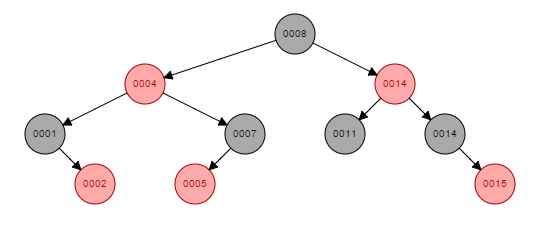
\includegraphics[width=.8\textwidth]{img/rbtree}
        \end{center}
    \end{solution}
  \end{questions}
\end{document}
